\documentclass[runningheads]{llncs}
\usepackage{graphicx}
\usepackage{amsmath,amssymb}
\usepackage{booktabs}
\usepackage{multirow}
\usepackage{makecell}
\usepackage{array}
\newcolumntype{L}[1]{>{\raggedright\arraybackslash}p{#1}}
\usepackage{xcolor}
\usepackage{pifont}
\usepackage{tikz}
\usetikzlibrary{positioning,arrows.meta,fit,backgrounds,calc,shapes.misc}
\usepackage[ruled,vlined,linesnumbered]{algorithm2e}
\usepackage{cite}
\usepackage{hyperref}

% ---------- draft helpers ----------
\newcommand{\tbd}[1]{\textcolor{red}{#1}}
\newcommand{\x}{\tbd{x.xxx}}
\newcommand{\cmark}{\ding{51}}
\newcommand{\xmark}{\ding{55}}
\newcommand{\pmark}{$\triangle$}
\newcommand{\figplaceholder}[2]{%
  \fbox{\begin{minipage}[c][#1][c]{0.92\textwidth}\centering
  \textcolor{red}{\small [Figure placeholder]\\ #2}\end{minipage}}}

\definecolor{contrib}{HTML}{C0392B}
\definecolor{contribfill}{HTML}{FADBD8}
\definecolor{basefill}{HTML}{EAF2F8}
\definecolor{basedraw}{HTML}{5D6D7E}

\begin{document}

\title{TB-HTL: Two-Branch Heterogeneous Transfer Learning for Workforce Attrition Risk Prediction across Heterogeneous HR Data Sources\thanks{\textcolor{red}{Draft. Values and statements in red are placeholders to be completed or verified after the experiments.}}}
\titlerunning{TB-HTL for Cross-Source Attrition Risk Prediction}

\maketitle

\begin{abstract}
Employee attrition imposes substantial replacement, productivity, and knowledge-loss costs on organizations, which has made attrition risk prediction a central task of HR analytics. In practice, however, HR data are collected by heterogeneous systems, such as internal HR information systems and external recruitment or learning platforms, whose schemas differ and whose labels capture different stages of the withdrawal process, from the intention to change jobs to actual attrition. Existing attrition models are trained and evaluated within a single dataset, so they cannot be reused across sources, and organizations with small or newly collected data cannot benefit from larger related sources. Our preliminary analysis shows that restricting models to the attributes shared by two public HR sources costs 0.21--0.23 AUC-ROC within each source, and that zero-shot transfer from the job-change source to the attrition target falls to chance level (AUC-ROC 0.498). To address this problem, this study proposes TB-HTL, a Two-Branch Heterogeneous Transfer Learning framework. TB-HTL aligns semantically equivalent HR attributes through canonical feature mapping with within-domain quantile alignment, pre-trains a shared canonical branch together with a source-private branch regularized by stochastic branch dropout, and transfers only the shared branch to the target, where it is fine-tuned with a new target-private branch using an anchored, label-shift-aware strategy. The framework outputs an attrition risk score accompanied by SHAP explanations. With only \tbd{$k=100$} labeled target employees, TB-HTL achieves a PR-AUC of \tbd{[x.xxx]} on the IBM attrition target, improving over the strongest target-only baseline by \tbd{[x.x]}\% and over canonical-only fine-tuning by \tbd{[x.x]}\%, while stochastic branch dropout contributes \tbd{[x.xxx]} PR-AUC. These results indicate that knowledge can be transferred between heterogeneous HR sources even when their labels differ in meaning.
\keywords{Transfer learning; Domain adaptation; Employee attrition; Heterogeneous tabular data; HR analytics; Explainable AI.}
\end{abstract}

%=====================================================================
\section{Introduction}
Employee attrition prediction is a binary classification task in which a model estimates, from demographic, job-related, and organizational attributes, whether an individual will leave their current position. The task has high practical value: replacing an experienced employee incurs recruitment, onboarding, and productivity costs that are commonly estimated to reach a large fraction of, or even exceed, the employee's annual salary \tbd{[citation needed]}. Consequently, machine learning has been applied to attrition prediction for two decades, from early neural networks~\cite{sexton2005} and churn models~\cite{saradhi2011} to classical classifiers~\cite{jain2020}, ensembles~\cite{alsheref2022,chung2023}, transformers~\cite{li2023}, and explainable pipelines~\cite{mohiuddin2023,baydili2025,alali2026}.

Despite this progress, nearly all existing studies implicitly assume that training and deployment data come from the same employee population. This assumption rarely holds in modern organizations, which collect HR data through heterogeneous systems: internal HR information systems record current employees, whereas recruitment and learning platforms record candidates and learners. These sources differ in schema, scale, and encoding, and their labels describe different stages of the same withdrawal process: the intention to change jobs precedes actual attrition~\cite{mobley1977}, and turnover intention is one of the strongest predictors of turnover behavior~\cite{griffeth2000}. Even the most recent studies that use several HR datasets~\cite{baydili2025,alali2026} train and evaluate a separate model on each dataset, and none examines whether a model learned from one source generalizes to another. As a result, organizations with small or newly collected HR data cannot benefit from larger related sources, and models deployed on a different population may fail silently. Our preliminary analysis on two public sources (Section~\ref{sec:gap}) confirms the severity of this problem: restricting models to the shared attributes alone costs 0.21--0.23 AUC-ROC within each source, and zero-shot transfer from the job-change source to the attrition target drops to AUC-ROC 0.498, a statistically significant degradation ($p=0.0016$).

Transfer learning and domain adaptation offer principled tools for this setting~\cite{pan2010,zhuang2021}, but existing techniques do not match its characteristics. Classical domain adaptation methods such as CORAL~\cite{sun2016} and DANN~\cite{ganin2015} assume a shared feature space and an identical task, whereas the two HR sources differ in both. Supervised pre-training and fine-tuning for tabular data~\cite{levin2023} is effective when upstream and downstream tasks share the same columns, but handles only a few missing features. Cross-table models such as TransTab~\cite{wang2022} and CARTE~\cite{kim2024} accept different columns but rely on column-name semantics rather than on explicit alignment of value scales, and are not designed for a shift in label meaning. Tabular foundation models such as TabPFN~\cite{hollmann2025} predict well on small datasets but ignore related source data. Motivated by these limitations, this study addresses the following research questions:
\begin{itemize}
\item \textbf{RQ1:} How can semantically equivalent but differently encoded HR attributes be aligned across heterogeneous sources?
\item \textbf{RQ2:} How can a transfer model exploit the features unique to each source instead of only the attributes they share?
\item \textbf{RQ3:} How can the shared representation remain transferable when source-specific features dominate the pre-training signal?
\item \textbf{RQ4:} How can a pre-trained model adapt to a target label with a different meaning using only a few labeled target samples?
\end{itemize}

To answer these questions, this study proposes TB-HTL, a Two-Branch Heterogeneous Transfer Learning framework for cross-source attrition risk prediction. TB-HTL maps both sources onto a set of canonical HR concepts, pre-trains a two-branch network on the source, transfers only its canonical branch, and fine-tunes it together with a new target-specific branch on a few labeled target employees. The main contributions of this study are summarized as follows:
\begin{itemize}
\item A canonical feature mapping with within-domain quantile alignment is proposed to place semantically equivalent HR attributes on a common, distribution-aligned scale.
\item A two-branch heterogeneous architecture is proposed that pre-trains on all source features and fine-tunes on all target features, while transferring only the shared canonical branch.
\item A stochastic private-branch dropout strategy is proposed to force the canonical branch to carry predictive information during pre-training, which makes it transferable.
\item An anchored, label-shift-aware fine-tuning strategy is proposed to adapt the transferred representation to a target label with different semantics using only a few labeled samples; the resulting model provides attrition risk scores with SHAP explanations.
\end{itemize}

The remainder of this paper is organized as follows. Section~\ref{sec:related} reviews related work on attrition prediction and transfer learning for tabular data. Section~\ref{sec:method} presents the proposed TB-HTL framework. Section~\ref{sec:exp} describes the experimental setup and discusses the results. Finally, Section~\ref{sec:concl} concludes the paper and outlines future research directions.

%=====================================================================
\section{Related Work}\label{sec:related}
Research on attrition prediction has progressed from improving accuracy on a single dataset toward explainability and multi-dataset evaluation, whereas research on transfer learning for tabular data has progressed from domain adaptation in a shared feature space toward models that accept different columns. To position this study at the intersection of the two lines, representative methods were reviewed, ranging from classical domain adaptation (2015--2016) to the most recent attrition and tabular foundation models (2022--2026). As summarized in Table~\ref{tab:rw1}, these methods differ in the data sources they use, the feature spaces they assume, whether target labels are used, and the transfer mechanism. From these mechanisms, five core characteristics can be identified: cross-source transfer, support for heterogeneous schemas, explicit value-scale alignment of shared concepts, adaptation to a shifted label with few target labels, and explainable risk output. These characteristics provide the basis for the comparison in Table~\ref{tab:rw2}.

\begin{table}[t]
\centering
\caption{Comparison of data settings and transfer mechanisms in representative studies.}\label{tab:rw1}
\scriptsize
\setlength{\tabcolsep}{3pt}
\begin{tabular}{@{}L{2.9cm}L{2.2cm}L{1.4cm}cL{3.85cm}@{}}
\toprule
Study & Data sources & \makecell[l]{Feature\\space} & \makecell{Target\\labels} & Transfer mechanism (backbone) \\
\midrule
DANN (2015)~\cite{ganin2015} & Source + target & Shared & \xmark & Adversarial feature alignment (neural network) \\
CORAL (2016)~\cite{sun2016} & Source + target & Shared & \xmark & Covariance alignment (any classifier) \\
TransTab (2022)~\cite{wang2022} & Multiple tables & Partially shared & \cmark & Column-name tokenization, pre-training + fine-tuning (transformer) \\
Levin et al. (2023)~\cite{levin2023} & One table, many tasks & Shared & \cmark & Supervised pre-training + fine-tuning (MLP, FT-Transformer) \\
CARTE (2024)~\cite{kim2024} & Multiple tables & Different & \cmark & Graph pre-training + fine-tuning (graph transformer) \\
TabPFN v2 (2025)~\cite{hollmann2025} & Target only & Any & \cmark & In-context learning with a synthetic prior (transformer) \\
Baydili \& Tasci (2025)~\cite{baydili2025} & 2 HR datasets, separately & Per dataset & \cmark & None (GAN + transformer, SHAP) \\
AL-Ali et al. (2026)~\cite{alali2026} & 4 HR datasets, separately & Per dataset & \cmark & None (ML/DL models, SHAP) \\
\midrule
\textbf{TB-HTL (ours)} & \textbf{2 HR sources, jointly} & \textbf{Different} & \cmark & \textbf{Canonical-branch transfer with private branches (two-branch MLP, SHAP)} \\
\bottomrule
\end{tabular}
\end{table}

\begin{table}[t]
\centering
\caption{Comparison of core characteristics of representative methods. \cmark: supported; \pmark: partially supported; \xmark: not supported.}\label{tab:rw2}
\scriptsize
\setlength{\tabcolsep}{3.5pt}
\begin{tabular}{@{}lccccc@{}}
\toprule
Study & \makecell{Cross-source\\transfer} & \makecell{Heterogeneous\\schemas} & \makecell{Value-scale\\alignment} & \makecell{Label-shift\\adaptation} & \makecell{Explainable\\risk output} \\
\midrule
DANN (2015)~\cite{ganin2015} & \cmark & \xmark & \xmark & \xmark & \xmark \\
CORAL (2016)~\cite{sun2016} & \cmark & \xmark & \pmark & \xmark & \xmark \\
TransTab (2022)~\cite{wang2022} & \cmark & \cmark & \xmark & \pmark & \xmark \\
Levin et al. (2023)~\cite{levin2023} & \cmark & \pmark & \xmark & \cmark & \xmark \\
CARTE (2024)~\cite{kim2024} & \cmark & \cmark & \xmark & \pmark & \xmark \\
TabPFN v2 (2025)~\cite{hollmann2025} & \xmark & \xmark & \xmark & \xmark & \xmark \\
Baydili \& Tasci (2025)~\cite{baydili2025} & \xmark & \xmark & \xmark & \xmark & \cmark \\
AL-Ali et al. (2026)~\cite{alali2026} & \xmark & \xmark & \xmark & \xmark & \cmark \\
\midrule
\textbf{TB-HTL (ours)} & \cmark & \cmark & \cmark & \cmark & \cmark \\
\bottomrule
\end{tabular}
\end{table}

As indicated by Tables~\ref{tab:rw1} and~\ref{tab:rw2}, recent studies have improved specific aspects of the problem, but several limitations remain. Attrition studies that use multiple HR datasets~\cite{baydili2025,alali2026} evaluate each dataset independently and therefore provide no cross-source transfer. Classical domain adaptation~\cite{ganin2015,sun2016} aligns feature distributions without target labels, but requires a shared feature space and assumes that the conditional distribution of the label is unchanged, which contradicts the shift from job-change intention to realized attrition. Supervised tabular transfer~\cite{levin2023} explicitly handles a different downstream task, but assumes that upstream and downstream data share their columns and recovers only a few missing features through pseudo-features. Cross-table models~\cite{wang2022,kim2024} accept heterogeneous columns, but they align attributes through column names and language embeddings rather than through the meaning and scale of their values, so equivalent concepts with different encodings (e.g., a 1--5 education code versus education-level strings) are not explicitly aligned. Tabular foundation models~\cite{hollmann2025} predict well on small target sets but cannot exploit a related labeled source. Therefore, no existing method simultaneously supports cross-source transfer between heterogeneous HR schemas, explicit alignment of shared HR concepts, adaptation to a shifted label with few target samples, and explainable risk output within a unified framework. These limitations motivate the proposed TB-HTL framework, whose components are designed to cover all five characteristics in Table~\ref{tab:rw2}.

%=====================================================================
\section{TB-HTL Method}\label{sec:method}
\subsection{Problem Formulation}
Let $\mathcal{D}_S=\{(\mathbf{x}^S_i,y^S_i)\}_{i=1}^{n_S}$ denote a labeled source domain and $\mathcal{D}_T$ a target domain of which only $k\ll n_T$ samples are labeled. The two domains have different feature spaces, $\mathcal{X}_S\neq\mathcal{X}_T$, and binary labels with different semantics: in this study, the source label indicates the intention to change jobs and the target label indicates realized attrition (or vice versa), so that $P_S(y\mid\mathbf{x})\neq P_T(y\mid\mathbf{x})$ in general. Because the tasks differ and a few target labels are available, the setting is an instance of inductive transfer learning~\cite{pan2010}, as opposed to transductive domain adaptation, which assumes an identical task. Domain adaptation theory~\cite{bendavid2010} bounds the target error by the source error, a divergence between the input distributions, and the error of the best joint hypothesis; the last term grows when the labeling functions of the two domains differ, so aligning the input distributions alone cannot guarantee transfer under a shift in label meaning. We assume a small set of concepts $\mathcal{C}$ that are semantically meaningful in both domains. Each sample is decomposed as $\mathbf{x}^d=[\mathbf{c}^d,\mathbf{p}^d]$, where $\mathbf{c}^d=\phi_d(\mathbf{x}^d)\in\mathbb{R}^{m}$ is its canonical representation and $\mathbf{p}^d$ contains the private features available only in domain $d\in\{S,T\}$.

\subsection{Overview}
\begin{figure}[t]
\centering
\resizebox{\textwidth}{!}{%
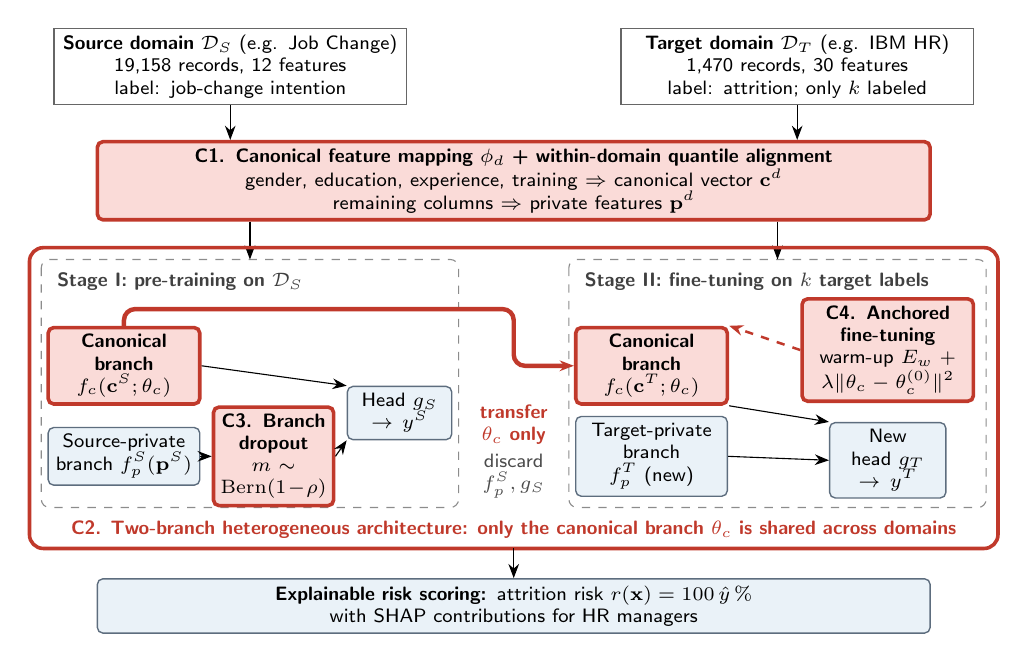
\begin{tikzpicture}[
  font=\sffamily\scriptsize,
  >={Stealth[length=1.8mm]},
  base/.style={draw=basedraw, fill=basefill, rounded corners=2pt, align=center, inner sep=2.5pt, line width=0.5pt},
  contr/.style={draw=contrib, fill=contribfill, rounded corners=2pt, align=center, inner sep=2.5pt, line width=1.3pt, font=\sffamily\scriptsize\bfseries},
  data/.style={draw=black!60, fill=white, align=center, inner sep=2.5pt, line width=0.5pt},
  stage/.style={draw=black!45, dashed, rounded corners=3pt},
  ttl/.style={font=\sffamily\scriptsize\bfseries, text=black!75, anchor=north west, align=left},
  nb/.style={font=\sffamily\scriptsize\mdseries}
]
% ---------- data
\node[data, text width=4.3cm] (src) at (2.4,0) {\textbf{Source domain $\mathcal{D}_S$} (e.g. Job Change)\\ 19,158 records, 12 features\\ label: job-change intention};
\node[data, text width=4.3cm] (tgt) at (9.6,0) {\textbf{Target domain $\mathcal{D}_T$} (e.g. IBM HR)\\ 1,470 records, 30 features\\ label: attrition; only $k$ labeled};
% ---------- C1
\node[contr, text width=10.4cm] (map) at (6.0,-1.45) {C1. Canonical feature mapping $\phi_d$ + within-domain quantile alignment\\[1pt]{\sffamily\mdseries gender, education, experience, training $\Rightarrow$ canonical vector $\mathbf{c}^d$\\ remaining columns $\Rightarrow$ private features $\mathbf{p}^d$}};
\draw[->] (src.south) -- (src.south |- map.north);
\draw[->] (tgt.south) -- (tgt.south |- map.north);
% ---------- stage boxes
\draw[stage] (0,-2.45) rectangle (5.3,-5.6);
\draw[stage] (6.7,-2.45) rectangle (12.0,-5.6);
\node[ttl] at (0.08,-2.5) {Stage I: pre-training on $\mathcal{D}_S$};
\node[ttl] at (6.78,-2.5) {Stage II: fine-tuning on $k$ target labels};
\draw[->] (2.65,0 |- map.south) -- (2.65,-2.45);
\draw[->] (9.35,0 |- map.south) -- (9.35,-2.45);
% ---------- Stage I
\node[contr, text width=1.75cm] (fcS) at (1.05,-3.8) {Canonical branch\\{\sffamily\mdseries $f_c(\mathbf{c}^S;\theta_c)$}};
\node[base, text width=1.75cm] (fpS) at (1.05,-4.95) {Source-private\\branch $f_p^S(\mathbf{p}^S)$};
\node[contr, text width=1.35cm] (bd) at (2.95,-4.95) {C3. Branch\\dropout\\{\sffamily\mdseries $m\!\sim\!\mathrm{Bern}(1\!-\!\rho)$}};
\node[base, text width=1.15cm] (gS) at (4.55,-4.4) {Head $g_S$\\$\to y^S$};
\draw[->] (fpS) -- (bd);
\draw[->] (bd.east) -- (gS.south west);
\draw[->] (fcS.east) -- (gS.north west);
% ---------- Stage II
\node[contr, text width=1.75cm] (fcT) at (7.75,-3.8) {Canonical branch\\{\sffamily\mdseries $f_c(\mathbf{c}^T;\theta_c)$}};
\node[base, text width=1.75cm] (fpT) at (7.75,-4.95) {Target-private\\branch $f_p^T$ (new)};
\node[contr, text width=2.0cm] (anc) at (10.75,-3.6) {C4. Anchored fine-tuning\\{\sffamily\mdseries warm-up $E_w$ + $\lambda\|\theta_c-\theta_c^{(0)}\|^2$}};
\node[base, text width=1.3cm] (gT) at (10.75,-5.0) {New head $g_T$\\$\to y^T$};
\draw[->] (fcT.south east) -- (gT.north west);
\draw[->] (fpT.east) -- (gT.west);
\draw[->, dashed, contrib, line width=0.9pt] (anc.west) -- (fcT.north east);
% ---------- transfer (routed below the stage titles)
\draw[->, line width=1.6pt, contrib, rounded corners=4pt] (fcS.north) -- (1.05,-3.08) -- (6.0,-3.08) |- (fcT.west);
\node[font=\sffamily\scriptsize\bfseries, text=contrib, align=center] at (6.0,-4.55) {transfer\\$\theta_c$ only};
\node[nb, text=black!70, align=center] at (6.0,-5.2) {discard\\$f_p^S, g_S$};
% ---------- C2 frame
\node[font=\sffamily\scriptsize\bfseries, text=contrib] at (6.0,-5.88) {C2. Two-branch heterogeneous architecture: only the canonical branch $\theta_c$ is shared across domains};
\draw[contrib, line width=1.3pt, rounded corners=5pt] (-0.15,-2.3) rectangle (12.15,-6.12);
% ---------- output
\node[base, text width=10.4cm] (out) at (6.0,-6.85) {\textbf{Explainable risk scoring:} attrition risk \mbox{$r(\mathbf{x})=100\,\hat{y}\,\%$} with SHAP contributions for HR managers};
\draw[->] (6.0,-6.12) -- (out.north);
\end{tikzpicture}}
\caption{Overview of the proposed TB-HTL framework. Components outlined in bold red (C1--C4) are the main contributions of this study.}\label{fig:overview}
\end{figure}

Figure~\ref{fig:overview} illustrates the overall workflow of TB-HTL. Both domains are first mapped onto the canonical concepts by the canonical feature mapping, which also aligns the value scales of these concepts within each domain. A two-branch network is then pre-trained on the source domain: the canonical branch encodes the shared concepts, the source-private branch encodes the remaining source features, and stochastic branch dropout prevents the network from relying exclusively on the private features. After pre-training, only the canonical branch is transferred; the source-private branch and the source head are discarded. On the target domain, the transferred branch is combined with a new target-private branch and a new head and fine-tuned on the $k$ labeled target samples using an anchored, label-shift-aware strategy. The fine-tuned model produces an attrition risk score for each employee together with SHAP explanations.

\begin{algorithm}[t]
\caption{TB-HTL}\label{alg:tbhtl}
\small
\KwIn{Source data $\mathcal{D}_S$; labeled target subset $\mathcal{D}_T^{k}$; mappings $\phi_S,\phi_T$; dropout rate $\rho$; anchor weight $\lambda$; warm-up epochs $E_w$; learning rates $\eta,\eta_c$}
\KwOut{Fine-tuned target model $(f_c,f_p^T,g_T)$ and risk scoring function $r(\cdot)$}
\tcp{C1: canonical feature mapping}
\ForEach{domain $d\in\{S,T\}$}{
  Encode the canonical concepts of $\mathbf{x}^d$ and align their scales with Eq.~(\ref{eq:qt}) fitted on the training split of $d$\;
  Split each sample into $\mathbf{c}^d=\phi_d(\mathbf{x}^d)$ and private features $\mathbf{p}^d$\;
}
\tcp{Stage I: pre-training with C2 + C3}
Initialize $f_c$, $f_p^S$, $g_S$; hold out a source validation split\;
\While{validation PR-AUC improves (early stopping)}{
  \ForEach{mini-batch $\{(\mathbf{c}_i,\mathbf{p}_i,y_i)\}$ of $\mathcal{D}_S$}{
    Sample masks $m_i\sim\mathrm{Bernoulli}(1-\rho)$\;
    Compute $\hat{y}_i$ with Eq.~(\ref{eq:twobranch}) and update all parameters with the weighted loss Eq.~(\ref{eq:wbce})\;
  }
}
Store $\theta_c^{(0)}\leftarrow\theta_c$; discard $f_p^S$ and $g_S$\;
\tcp{Stage II: anchored fine-tuning (C4)}
Initialize a new private branch $f_p^T$ and a new head $g_T$\;
\For{$e=1$ \KwTo $E$}{
  \lIf{$e\le E_w$}{freeze $\theta_c$; update $f_p^T,g_T$ with rate $\eta$}
  \lElse{update $\theta_c$ with rate $\eta_c<\eta$ and $f_p^T,g_T$ with rate $\eta$ using Eq.~(\ref{eq:anchor})}
}
\Return{fine-tuned model and $r(\mathbf{x})$ of Eq.~(\ref{eq:risk}) with SHAP values}\;
\end{algorithm}

Algorithm~\ref{alg:tbhtl} summarizes the procedure. The algorithm first applies the canonical feature mapping to both domains, fitting all transformations on training splits only. During pre-training, each mini-batch of source samples is passed through both branches, a Bernoulli mask randomly removes the contribution of the private branch for each sample, and all parameters are updated with a class-weighted loss until the validation PR-AUC stops improving. The canonical branch parameters are then stored as the anchor $\theta_c^{(0)}$. During fine-tuning, the new target-private branch and head are first trained while the canonical branch is frozen; afterwards, all parameters are trained jointly, with a smaller learning rate and an anchoring penalty on the canonical branch. The final model returns the risk score and its SHAP explanation.

\subsection{Core Components}
\paragraph{C1. Canonical Feature Mapping with Quantile Alignment.}
The two sources record four common HR concepts with different encodings: gender, education level, years of working experience, and participation in training. The mapping $\phi_d$ first encodes each concept on a common semantic scale: gender is encoded as a binary indicator with an additional flag for other or missing values; education is mapped to a shared five-level ordinal scale (e.g., \emph{Below College}/\emph{High School}$\to1$, \emph{Bachelor}/\emph{Graduate}$\to3$, \emph{Master}$\to4$, \emph{Doctor}/\emph{PhD}$\to5$); experience is converted to years and capped; training is kept as recorded (number of trainings per year versus hours of training). Because the same concept may have different units and distributions in the two domains, each continuous or ordinal concept $v$ is then aligned by its within-domain rank:
\begin{equation}\label{eq:qt}
\tilde{v}=\Phi^{-1}\!\big(\hat{F}_d(v)\big),
\end{equation}
where $\hat{F}_d$ is the empirical cumulative distribution function of $v$ fitted on the training split of domain $d$ and $\Phi^{-1}$ is the standard normal quantile function. Eq.~(\ref{eq:qt}) maps the concept to a standard normal scale in both domains, so that values with the same relative position (e.g., an employee in the top 10\% of training participation) receive the same canonical value. This preserves the ordering information that is comparable across sources while removing scale differences that are not.

\paragraph{C2. Two-Branch Heterogeneous Architecture.}
Restricting a transfer model to $\mathbf{c}^d$ discards most of the information in each source (Section~\ref{sec:gap}). TB-HTL therefore uses two branches: a canonical encoder $f_c:\mathbb{R}^{m}\to\mathbb{R}^{h}$ with parameters $\theta_c$, which is shared across domains, and a private encoder $f_p^d:\mathbb{R}^{|\mathbf{p}^d|}\to\mathbb{R}^{h}$, which is specific to domain $d$. The prediction for sample $i$ is
\begin{equation}\label{eq:twobranch}
\hat{y}_i=\sigma\!\Big(g_d\big(\big[\,f_c(\mathbf{c}_i)\,;\,m_i\cdot f_p^d(\mathbf{p}_i)\,\big]\big)\Big),
\end{equation}
where $[\,\cdot\,;\,\cdot\,]$ denotes concatenation, $g_d$ is a domain-specific head, $\sigma$ is the sigmoid function, and $m_i\in\{0,1\}$ is a branch mask that equals 1 at inference time. Pre-training uses all source features through $f_c$ and $f_p^S$, and fine-tuning uses all target features through $f_c$ and $f_p^T$; only $\theta_c$ is transferred. Unlike pseudo-feature imputation~\cite{levin2023}, which must predict every column missing from the source and is feasible only for a few columns, this design never imputes the 8--26 private features of each domain.

\paragraph{C3. Stochastic Private-Branch Dropout.}
When the private features are more predictive than the canonical ones, the head can ignore $f_c$ during pre-training, leaving little transferable knowledge in $\theta_c$. To prevent this, the mask in Eq.~(\ref{eq:twobranch}) is sampled per sample as $m_i\sim\mathrm{Bernoulli}(1-\rho)$ during pre-training, where $\rho\in[0,1)$ is the branch dropout rate. With probability $\rho$, the network must predict the source label from the canonical branch alone, which forces $f_c$ to encode predictive information. The pre-training objective is the class-weighted binary cross-entropy
\begin{equation}\label{eq:wbce}
\mathcal{L}_S=-\frac{1}{n_S}\sum_{i=1}^{n_S}\Big[w_{+}\,y_i\log\hat{y}_i+(1-y_i)\log(1-\hat{y}_i)\Big],\qquad w_{+}=\frac{n_{-}}{n_{+}},
\end{equation}
where $n_{+}$ and $n_{-}$ denote the numbers of positive and negative training samples; the weight $w_{+}$ compensates for class imbalance.

\paragraph{C4. Anchored Label-Shift-Aware Fine-Tuning.}
Because the target label differs in meaning from the source label, the source head encodes a mapping that should not be reused. TB-HTL therefore re-initializes the head $g_T$ and the private branch $f_p^T$, and reuses only the representation $f_c$, whose risk factors (e.g., experience and training) are expected to be shared across the withdrawal process~\cite{mobley1977,griffeth2000}. Fine-tuning proceeds in two phases. During the first $E_w$ epochs, $\theta_c$ is frozen so that the randomly initialized modules do not distort the transferred representation. Afterwards, all parameters are trained with a smaller learning rate $\eta_c<\eta$ for $\theta_c$ and the anchored objective
\begin{equation}\label{eq:anchor}
\mathcal{L}_T=\mathcal{L}_{\mathrm{BCE}}\big(\mathcal{D}_T^{k}\big)+\lambda\,\big\|\theta_c-\theta_c^{(0)}\big\|_2^2,
\end{equation}
where $\mathcal{L}_{\mathrm{BCE}}$ is the class-weighted loss of Eq.~(\ref{eq:wbce}) on the $k$ labeled target samples and the second term, the L2-SP penalty~\cite{li2018}, keeps $\theta_c$ close to its pre-trained value $\theta_c^{(0)}$. With small $k$, the penalty prevents the canonical branch from over-fitting the few target labels; with larger $k$, the data term dominates and the representation can adapt.

\paragraph{Explainable Risk Scoring.}
For an employee $\mathbf{x}$, the framework outputs the risk score
\begin{equation}\label{eq:risk}
r(\mathbf{x})=100\cdot\hat{y}(\mathbf{x})\ \%,
\end{equation}
together with SHAP values~\cite{lundberg2017} that decompose the prediction into the contributions of individual features. Aggregating the absolute SHAP values of the canonical concepts in the source and target models also allows us to measure whether the same risk factors drive both labels.

%=====================================================================
\section{Experiment and Result}\label{sec:exp}
\subsection{Experimental Setup}
\paragraph{Datasets.} Experiments are conducted on two public HR sources. Domain~A is the IBM HR Analytics Employee Attrition \& Performance dataset, a fictional dataset created by IBM data scientists~\cite{alali2026}, containing 1,470 employees, 30 features after removing constant and identifier columns, and the label \emph{Attrition} (realized attrition, about 16\% positive). Domain~B is the HR Analytics: Job Change of Data Scientists dataset, containing 19,158 labeled records, 12 features, and the label \emph{target} (intention to change jobs, about \tbd{25}\% positive). The four canonical concepts are gender, education level, years of experience, and training participation; the remaining 26 features of A and 8 features of B are private. Both transfer directions are evaluated: B$\to$A, where a large source supports a small target, is the main setting, and A$\to$B is evaluated for completeness.

\paragraph{Preprocessing.} Missing numerical values are imputed with the median and missing categorical values with a new category, using statistics from the training split only. Private categorical features are one-hot encoded, private numerical features are standardized, and canonical concepts are processed by C1. For each of 10 random seeds, the target domain is split into 80\% training and 20\% test sets with stratification, and $k\in\{20,50,100,200,500,\text{All}\}$ labeled samples are drawn from the target training set by stratified sampling with at least one positive sample; ``All'' denotes the full target training set (1,176 for A and about 15,326 for B). The full source domain is used for pre-training, with 10\% held out for early stopping.

\paragraph{Baselines.} The baselines follow the methods reviewed in Table~\ref{tab:rw1}. \emph{Target-only} baselines are trained on the $k$ target samples: logistic regression (LR), random forest (RF), XGBoost, and TabPFN v2~\cite{hollmann2025}, the most recent tabular foundation model for small data. \emph{Unsupervised transfer} baselines use no target labels: zero-shot transfer (a source RF applied to the canonical features), CORAL~\cite{sun2016}, and DANN~\cite{ganin2015}. \emph{Supervised transfer} baselines use the same $k$ target labels: canonical-only fine-tuning following Levin et al.~\cite{levin2023} (FT-Canonical), TransTab~\cite{wang2022}, and CARTE~\cite{kim2024}. The in-domain models of the multi-dataset attrition studies~\cite{baydili2025,alali2026} correspond to the target-only setting with all target labels.

\paragraph{Model Settings.} Table~\ref{tab:config} summarizes the configurations. Hyperparameters of the target-only baselines are tuned by stratified 5-fold cross-validation on the available target samples when $k\ge100$ and fixed to library defaults otherwise, because very small $k$ does not support reliable validation~\cite{levin2023}.

\begin{table}[t]
\centering
\caption{Experimental configuration of the baselines and TB-HTL. \tbd{Values to be finalized during the experiments.}}\label{tab:config}
\scriptsize
\setlength{\tabcolsep}{3pt}
\begin{tabular}{@{}lL{8.0cm}@{}}
\toprule
Method & Parameters \\
\midrule
LR & L2 penalty; $C\in\{0.01,0.1,1,10,100\}$; class\_weight = balanced \\
RF & 300 trees; class\_weight = balanced \\
XGBoost & 300 trees; max depth $\in\{3,5,7\}$; scale\_pos\_weight $=n_-/n_+$ \\
TabPFN v2~\cite{hollmann2025} & Default in-context configuration \\
Zero-shot / CORAL~\cite{sun2016} & RF on canonical features; CORAL regularization $=1$ \\
DANN~\cite{ganin2015} & Same MLP backbone as TB-HTL; gradient reversal with the schedule of~\cite{ganin2015} \\
FT-Canonical~\cite{levin2023} & MLP on canonical features; supervised pre-training; MLP-head end-to-end fine-tuning \\
TransTab~\cite{wang2022}, CARTE~\cite{kim2024} & Default configurations of the official implementations \\
\midrule
\textbf{TB-HTL} & Encoders: MLP $2\times128$, ReLU, dropout 0.1; head: MLP 128; AdamW, $\eta=10^{-3}$, weight decay $10^{-5}$, batch 256; pre-training $\le$200 epochs, patience 20; $\rho=\tbd{0.4}$; fine-tuning: $E_w=10$, $\eta_c=10^{-4}$, $\lambda=\tbd{10^{-2}}$, 30 epochs ($k\le50$), 60 epochs ($k\le200$), early stopping on 20\% validation ($k\ge500$) \\
\bottomrule
\end{tabular}
\end{table}

\paragraph{Environment.} All experiments are conducted on Google Colaboratory with \tbd{an NVIDIA T4 GPU} using Python~3.10, PyTorch, scikit-learn, XGBoost, imbalanced-learn, and SHAP.

\paragraph{Evaluation Metrics.} Because both labels are imbalanced, PR-AUC is the primary metric, as it is threshold-independent and sensitive to the minority class. AUC-ROC, F1-score, and G-Mean ($\sqrt{\mathrm{TPR}\cdot\mathrm{TNR}}$) are secondary metrics; accuracy is not reported. Thresholds for F1-score and G-Mean are selected without using the target test set (on the source validation split for unsupervised transfer, and on the $k$ target samples for supervised transfer), since the positive rates of the two domains differ. All results are reported as mean $\pm$ standard deviation over 10 seeds, and differences are tested with the paired $t$-test and the Wilcoxon signed-rank test at $\alpha=0.05$.

\paragraph{Validation Protocol.} Four experiments correspond to the four components. C1 is evaluated by comparing alternative canonical encodings in terms of the mean one-dimensional Wasserstein distance between source and target canonical features and the zero-shot PR-AUC. C2 is evaluated by comparing TB-HTL with target-only and supervised transfer baselines across all values of $k$. C3 is evaluated by an ablation on the pre-training strategy, including the PR-AUC of the canonical branch alone on the source validation split. C4 is evaluated by comparing unsupervised transfer with several fine-tuning strategies. Finally, the overall evaluation covers both directions, stability, computational cost, class-imbalance handling (class weighting versus SMOTE~\cite{chawla2002}, ADASYN~\cite{he2008}, and CTGAN~\cite{xu2019}), and the consistency of SHAP explanations.

\subsection{Result}
\paragraph{Diagnosing the Cross-Source Gap.}\label{sec:gap}
Table~\ref{tab:gap} reports a preliminary $2\times2$ experiment with a random forest that separates the effect of feature reduction from the effect of domain shift. Restricting each source to the four canonical concepts reduces AUC-ROC from 0.796 to 0.581 in Domain~A and from 0.787 to 0.561 in Domain~B, i.e., by 0.21--0.23. In contrast, the additional loss caused by changing the domain is smaller and asymmetric: in the B$\to$A direction, AUC-ROC drops from 0.581 (in-domain, canonical) to 0.498 (paired $t$-test, $p=0.0016$), whereas in the A$\to$B direction the change from 0.561 to 0.567 is not significant ($p=0.102$). These results show that most of the gap is caused by discarding domain-specific information, which motivates C2, and that the label shift makes zero-shot transfer from intention to attrition no better than chance, which motivates C4.

\begin{table}[t]
\centering
\caption{Preliminary $2\times2$ analysis with random forest (mean $\pm$ std over 10 splits): full versus canonical features, in-domain versus cross-domain.}\label{tab:gap}
\scriptsize
\setlength{\tabcolsep}{4pt}
\begin{tabular}{@{}lcccc@{}}
\toprule
\multirow{2}{*}{Setting} & \multicolumn{2}{c}{Full features} & \multicolumn{2}{c}{4 canonical features} \\
\cmidrule(lr){2-3}\cmidrule(lr){4-5}
 & AUC-ROC & PR-AUC & AUC-ROC & PR-AUC \\
\midrule
In-domain A (30 features) & 0.796 $\pm$ 0.034 & 0.490 $\pm$ 0.058 & 0.581 $\pm$ 0.056 & 0.234 $\pm$ 0.041 \\
In-domain B (12 features) & 0.787 $\pm$ 0.005 & 0.523 $\pm$ 0.008 & 0.561 $\pm$ 0.009 & 0.300 $\pm$ 0.006 \\
Cross-domain B$\to$A & -- & -- & 0.498 $\pm$ 0.045 & 0.165 $\pm$ 0.019 \\
Cross-domain A$\to$B & -- & -- & 0.567 $\pm$ 0.008 & 0.303 $\pm$ 0.007 \\
\bottomrule
\end{tabular}
\end{table}

\paragraph{Effect of Canonical Feature Alignment (C1).}
Table~\ref{tab:c1} compares three encodings of the canonical concepts: raw shared columns with min--max scaling, the semantic ordinal mapping alone, and the proposed mapping with quantile alignment. The proposed mapping \tbd{[reduces / does not reduce]} the mean Wasserstein distance between source and target canonical features from \x{} to \x{} and \tbd{[improves / does not improve]} the zero-shot PR-AUC in the B$\to$A direction from \x{} to \x{}. \tbd{[Interpretation to be written after the results: whether aligning value scales reduces the covariate gap even though, as expected, it cannot remove the label shift.]}

\begin{table}[t]
\centering
\caption{Effect of the canonical encoding on the source--target distribution gap and zero-shot performance (RF).}\label{tab:c1}
\scriptsize
\setlength{\tabcolsep}{5pt}
\begin{tabular}{@{}lccc@{}}
\toprule
Canonical encoding & \makecell{Mean Wasserstein\\distance $\downarrow$} & \makecell{PR-AUC\\B$\to$A $\uparrow$} & \makecell{PR-AUC\\A$\to$B $\uparrow$} \\
\midrule
Raw shared columns (min--max) & \x & \x & \x \\
Semantic ordinal mapping & \x & \x & \x \\
\textbf{Semantic mapping + quantile alignment (C1)} & \x & \x & \x \\
\bottomrule
\end{tabular}
\end{table}

\paragraph{Effect of the Two-Branch Architecture (C2).}
Table~\ref{tab:c2} and Fig.~\ref{fig:curve} compare TB-HTL with target-only and supervised transfer baselines in the B$\to$A direction. With $k=100$ labeled target employees, TB-HTL reaches a PR-AUC of \x{}, compared with \x{} for the best target-only baseline (\tbd{[name]}) and \x{} for FT-Canonical. \tbd{[Describe the learning curves: the range of $k$ in which TB-HTL is significantly better, and the value of $k$ at which target-only models catch up; compare with the in-domain upper bound of 0.490 PR-AUC in Table~\ref{tab:gap}.]} The comparison with FT-Canonical isolates the benefit of exploiting private features, and the comparison with TransTab and CARTE isolates the benefit of explicit concept alignment over column-name-based alignment.

\begin{table}[t]
\centering
\caption{PR-AUC (mean $\pm$ std over 10 seeds) in the B$\to$A direction for different numbers $k$ of labeled target samples.}\label{tab:c2}
\scriptsize
\setlength{\tabcolsep}{2.6pt}
\begin{tabular}{@{}llcccccc@{}}
\toprule
Group & Method & $k=20$ & $k=50$ & $k=100$ & $k=200$ & $k=500$ & All \\
\midrule
\multirow{4}{*}{Target-only} & LR & \x & \x & \x & \x & \x & \x \\
 & RF & \x & \x & \x & \x & \x & \x \\
 & XGBoost & \x & \x & \x & \x & \x & \x \\
 & TabPFN v2~\cite{hollmann2025} & \x & \x & \x & \x & \x & \x \\
\midrule
\multirow{3}{*}{\makecell[l]{Supervised\\transfer}} & FT-Canonical~\cite{levin2023} & \x & \x & \x & \x & \x & \x \\
 & TransTab~\cite{wang2022} & \x & \x & \x & \x & \x & \x \\
 & CARTE~\cite{kim2024} & \x & \x & \x & \x & \x & \x \\
\midrule
Proposed & \textbf{TB-HTL} & \x & \x & \x & \x & \x & \x \\
\bottomrule
\end{tabular}
\end{table}

\begin{figure}[t]
\centering
\figplaceholder{3.2cm}{PR-AUC versus the number of labeled target samples $k$ (B$\to$A, log-scale $x$-axis), one line per method of Table~\ref{tab:c2}, with $\pm1$ std bands and the in-domain upper bound as a horizontal line.}
\caption{Learning curves of TB-HTL and the baselines in the B$\to$A direction.}\label{fig:curve}
\end{figure}

\paragraph{Effect of Stochastic Branch Dropout (C3).}
Table~\ref{tab:c3} reports an ablation on the pre-training strategy with $k=100$. Pre-training without branch dropout yields a canonical branch whose standalone source PR-AUC is \x{}, compared with \x{} when $\rho=\tbd{0.4}$. \tbd{[State whether the higher standalone quality of the canonical branch translates into higher target PR-AUC, and compare with pre-training on canonical features only, which is the strategy of FT-Canonical.]}

\begin{table}[t]
\centering
\caption{Ablation of the pre-training strategy ($k=100$). ``Canonical only'' denotes the PR-AUC of the canonical branch alone on the source validation split.}\label{tab:c3}
\scriptsize
\setlength{\tabcolsep}{4pt}
\begin{tabular}{@{}lcccc@{}}
\toprule
\multirow{2}{*}{Pre-training strategy} & \multicolumn{2}{c}{Source validation PR-AUC} & \multicolumn{2}{c}{Target test PR-AUC} \\
\cmidrule(lr){2-3}\cmidrule(lr){4-5}
 & Full model & Canonical only & B$\to$A & A$\to$B \\
\midrule
Canonical features only & -- & \x & \x & \x \\
Full features, no branch dropout ($\rho=0$) & \x & \x & \x & \x \\
Full features, $\rho=0.2$ & \x & \x & \x & \x \\
\textbf{Full features, $\rho=0.4$ (C3)} & \x & \x & \x & \x \\
Full features, $\rho=0.6$ & \x & \x & \x & \x \\
\bottomrule
\end{tabular}
\end{table}

\paragraph{Effect of Anchored Label-Shift-Aware Fine-Tuning (C4).}
Table~\ref{tab:c4} compares methods that do not use target labels with fine-tuning strategies that use $k$ target labels. Unsupervised alignment (CORAL and DANN) reaches a PR-AUC of \x{} in the B$\to$A direction, close to the zero-shot value of 0.165 and to the positive rate of the target domain \tbd{[to be confirmed]}, which is consistent with the hypothesis that aligning feature distributions cannot correct a change in label meaning. Among the fine-tuning strategies, the anchored strategy achieves \x{} with $k=50$, compared with \x{} for head-only fine-tuning and \x{} for unanchored full fine-tuning. \tbd{[Interpretation to be written after the results.]}

\begin{table}[t]
\centering
\caption{Unsupervised transfer versus fine-tuning strategies (PR-AUC, mean over 10 seeds).}\label{tab:c4}
\scriptsize
\setlength{\tabcolsep}{4pt}
\begin{tabular}{@{}llcccc@{}}
\toprule
\multirow{2}{*}{Target labels} & \multirow{2}{*}{Strategy} & \multicolumn{2}{c}{B$\to$A} & \multicolumn{2}{c}{A$\to$B} \\
\cmidrule(lr){3-4}\cmidrule(lr){5-6}
 & & $k=50$ & $k=200$ & $k=50$ & $k=200$ \\
\midrule
\multirow{3}{*}{None} & Zero-shot (RF) & 0.165$^{\dagger}$ & 0.165$^{\dagger}$ & 0.303$^{\dagger}$ & 0.303$^{\dagger}$ \\
 & CORAL~\cite{sun2016} & \x & \x & \x & \x \\
 & DANN~\cite{ganin2015} & \x & \x & \x & \x \\
\midrule
\multirow{3}{*}{$k$ labels} & Head-only fine-tuning (frozen $f_c$) & \x & \x & \x & \x \\
 & Full fine-tuning, no anchor ($\lambda=0$, no warm-up) & \x & \x & \x & \x \\
 & \textbf{Anchored fine-tuning (C4)} & \x & \x & \x & \x \\
\bottomrule
\multicolumn{6}{@{}l}{\scriptsize $^{\dagger}$ From Table~\ref{tab:gap}; independent of $k$ because no target labels are used.}
\end{tabular}
\end{table}

\paragraph{Overall Effectiveness of TB-HTL.}
Table~\ref{tab:overall} summarizes the overall performance in both directions together with computational cost. In the main B$\to$A direction with $k=100$, TB-HTL achieves a PR-AUC of \x{}, an AUC-ROC of \x{}, an F1-score of \x{}, and a G-Mean of \x{}. In the A$\to$B direction, where the source is smaller than the target, the gain is expected to be smaller, and TB-HTL achieves \x{} PR-AUC. Pre-training takes \tbd{[x]} s and fine-tuning \tbd{[x]} s per run, compared with \tbd{[x]} s for TransTab and \tbd{[x]} s for CARTE. For class imbalance, class weighting is compared with SMOTE~\cite{chawla2002}, ADASYN~\cite{he2008}, and CTGAN~\cite{xu2019} applied to the training data only; the best strategy is \tbd{[name]} with \x{} PR-AUC. Finally, Fig.~\ref{fig:shap} compares the SHAP importance of the canonical concepts in the source and target models; the Spearman correlation between the two rankings is \tbd{[x.xx]}, indicating that \tbd{[experience and education / other concepts]} are \tbd{[shared / not shared]} risk factors of job-change intention and realized attrition.

\begin{table}[t]
\centering
\caption{Overall comparison at $k=100$ (mean over 10 seeds) and computational cost per run.}\label{tab:overall}
\scriptsize
\setlength{\tabcolsep}{3pt}
\begin{tabular}{@{}llccccc@{}}
\toprule
Direction & Method & PR-AUC & AUC-ROC & F1-score & G-Mean & Time (s) \\
\midrule
\multirow{4}{*}{B$\to$A} & Best target-only (\tbd{[name]}) & \x & \x & \x & \x & \tbd{x} \\
 & FT-Canonical~\cite{levin2023} & \x & \x & \x & \x & \tbd{x} \\
 & Best cross-table (\tbd{TransTab/CARTE}) & \x & \x & \x & \x & \tbd{x} \\
 & \textbf{TB-HTL} & \x & \x & \x & \x & \tbd{x} \\
\midrule
\multirow{4}{*}{A$\to$B} & Best target-only (\tbd{[name]}) & \x & \x & \x & \x & \tbd{x} \\
 & FT-Canonical~\cite{levin2023} & \x & \x & \x & \x & \tbd{x} \\
 & Best cross-table (\tbd{TransTab/CARTE}) & \x & \x & \x & \x & \tbd{x} \\
 & \textbf{TB-HTL} & \x & \x & \x & \x & \tbd{x} \\
\bottomrule
\end{tabular}
\end{table}

\begin{figure}[t]
\centering
\figplaceholder{2.8cm}{Mean absolute SHAP values of the four canonical concepts in the source model (Job Change) and the target model (IBM), side by side, with an example of an individual risk explanation.}
\caption{Comparison of SHAP importance of the canonical concepts in the source and target models.}\label{fig:shap}
\end{figure}

%=====================================================================
\section{Conclusion}\label{sec:concl}
This paper proposed TB-HTL, a two-branch heterogeneous transfer learning framework for predicting workforce attrition risk across HR data sources whose schemas and labels differ. The framework integrates canonical feature mapping with quantile alignment, a two-branch architecture that transfers only the shared canonical branch, stochastic private-branch dropout during pre-training, and anchored label-shift-aware fine-tuning, and it outputs risk scores with SHAP explanations. A preliminary analysis on two public HR sources showed that discarding domain-specific features, rather than domain shift alone, causes most of the cross-source performance gap, and that zero-shot transfer from job-change intention to attrition is no better than chance. \tbd{[Summarize the main quantitative results of Tables~\ref{tab:c2}--\ref{tab:overall} in one or two sentences.]} Future work will extend the framework to more than two sources and to multi-task pre-training with auxiliary HR targets~\cite{caruana1997}, study unsupervised adaptation of the canonical branch when no target labels are available, and validate the approach on real organizational data rather than on public benchmark datasets.

\section*{Data and Code Availability}
The complete implementation will be made available at: \tbd{[repository link]}.

%=====================================================================
\begin{thebibliography}{99}

\bibitem{alali2026}
AL-Ali, M., et al.: Integrating machine learning and explainable AI for employee attrition prediction in HR analytics. Scientific Reports \textbf{16}, 6344 (2026)

\bibitem{alsheref2022}
Alsheref, F.K., Fattoh, I.E., Ead, W.M.: Automated prediction of employee attrition using ensemble model based on machine learning algorithms. Computational Intelligence and Neuroscience \textbf{2022}, 7728668 (2022)

\bibitem{baydili2025}
Baydili, \.{I}.T., Tasci, B.: Predicting employee attrition: XAI-powered models for managerial decision-making. Systems \textbf{13}(7), 583 (2025)

\bibitem{bendavid2010}
Ben-David, S., Blitzer, J., Crammer, K., Kulesza, A., Pereira, F., Vaughan, J.W.: A theory of learning from different domains. Machine Learning \textbf{79}(1--2), 151--175 (2010)

\bibitem{caruana1997}
Caruana, R.: Multitask learning. Machine Learning \textbf{28}(1), 41--75 (1997)

\bibitem{chawla2002}
Chawla, N.V., Bowyer, K.W., Hall, L.O., Kegelmeyer, W.P.: SMOTE: Synthetic minority over-sampling technique. Journal of Artificial Intelligence Research \textbf{16}, 321--357 (2002)

\bibitem{chung2023}
Chung, J., Yun, S., Lee, J., Jeon, H.: Predictive model of employee attrition based on stacking ensemble learning. Expert Systems with Applications \textbf{215}, 119364 (2023)

\bibitem{ganin2015}
Ganin, Y., Lempitsky, V.: Unsupervised domain adaptation by backpropagation. In: Proceedings of the 32nd International Conference on Machine Learning (ICML). pp. 1180--1189 (2015)

\bibitem{griffeth2000}
Griffeth, R.W., Hom, P.W., Gaertner, S.: A meta-analysis of antecedents and correlates of employee turnover: Update, moderator tests, and research implications for the next millennium. Journal of Management \textbf{26}(3), 463--488 (2000)

\bibitem{he2008}
He, H., Bai, Y., Garcia, E.A., Li, S.: ADASYN: Adaptive synthetic sampling approach for imbalanced learning. In: Proceedings of the IEEE International Joint Conference on Neural Networks (IJCNN). pp. 1322--1328 (2008)

\bibitem{hollmann2025}
Hollmann, N., Müller, S., Purucker, L., Krishnakumar, A., Körfer, M., Hoo, S.B., Schirrmeister, R.T., Hutter, F.: Accurate predictions on small data with a tabular foundation model. Nature \textbf{637}(8045), 319--326 (2025)

\bibitem{jain2020}
Jain, P.K., Jain, M., Pamula, R.: Explaining and predicting employees' attrition: a machine learning approach. SN Applied Sciences \textbf{2}, 757 (2020)

\bibitem{kim2024}
Kim, M.J., Grinsztajn, L., Varoquaux, G.: CARTE: Pretraining and transfer for tabular learning. In: Proceedings of the 41st International Conference on Machine Learning (ICML) (2024)

\bibitem{levin2023}
Levin, R., Cherepanova, V., Schwarzschild, A., Bansal, A., Bruss, C.B., Goldstein, T., Wilson, A.G., Goldblum, M.: Transfer learning with deep tabular models. In: International Conference on Learning Representations (ICLR) (2023)

\bibitem{li2023}
Li, W.: A transformer-based deep learning framework to predict employee attrition. PeerJ Computer Science \textbf{9}, e1570 (2023)

\bibitem{li2018}
Li, X., Grandvalet, Y., Davoine, F.: Explicit inductive bias for transfer learning with convolutional networks. In: Proceedings of the 35th International Conference on Machine Learning (ICML). pp. 2825--2834 (2018)

\bibitem{lundberg2017}
Lundberg, S.M., Lee, S.I.: A unified approach to interpreting model predictions. In: Advances in Neural Information Processing Systems (NeurIPS). vol.~30 (2017)

\bibitem{mobley1977}
Mobley, W.H.: Intermediate linkages in the relationship between job satisfaction and employee turnover. Journal of Applied Psychology \textbf{62}(2), 237--240 (1977)

\bibitem{mohiuddin2023}
Mohiuddin, K., et al.: Retention is all you need. In: Proceedings of the 32nd ACM International Conference on Information and Knowledge Management (CIKM). pp. 4752--4758 (2023)

\bibitem{pan2010}
Pan, S.J., Yang, Q.: A survey on transfer learning. IEEE Transactions on Knowledge and Data Engineering \textbf{22}(10), 1345--1359 (2010)

\bibitem{saradhi2011}
Saradhi, V.V., Palshikar, G.K.: Employee churn prediction. Expert Systems with Applications \textbf{38}(3), 1999--2006 (2011)

\bibitem{sexton2005}
Sexton, R.S., McMurtrey, S., Michalopoulos, J.O., Smith, A.M.: Employee turnover: a neural network solution. Computers \& Operations Research \textbf{32}(10), 2635--2651 (2005)

\bibitem{sun2016}
Sun, B., Feng, J., Saenko, K.: Return of frustratingly easy domain adaptation. In: Proceedings of the Thirtieth AAAI Conference on Artificial Intelligence. pp. 2058--2065 (2016)

\bibitem{wang2022}
Wang, Z., Sun, J.: TransTab: Learning transferable tabular transformers across tables. In: Advances in Neural Information Processing Systems (NeurIPS). vol.~35 (2022)

\bibitem{xu2019}
Xu, L., Skoularidou, M., Cuesta-Infante, A., Veeramachaneni, K.: Modeling tabular data using conditional GAN. In: Advances in Neural Information Processing Systems (NeurIPS). vol.~32 (2019)

\bibitem{zhuang2021}
Zhuang, F., Qi, Z., Duan, K., Xi, D., Zhu, Y., Zhu, H., Xiong, H., He, Q.: A comprehensive survey on transfer learning. Proceedings of the IEEE \textbf{109}(1), 43--76 (2021)

\end{thebibliography}
\end{document}
